\documentclass[letterpaper,12pt,oneside]{article}
\usepackage{hyperref}
%\pagestyle{headings}
\pagenumbering{arabic}

\setlength{\hoffset}{-1.5cm}
\setlength{\voffset}{-2cm}
\setlength{\textheight}{22.5cm}
\setlength{\textwidth}{17cm}
\renewcommand{\baselinestretch}{1.3}


%\VignetteIndexEntry{OneMap Tutorial}


\usepackage{Sweave}
\begin{document}

\begin{titlepage}
  {\LARGE {\bf OneMap Tutorial}}
  \medskip\hrule height 2pt
  \vspace{.08in}

  {\flushright Software for constructing genetic maps in experimental crosses: full-sib, RILs, F$_2$ and backcrosses}
  
  \vspace{.4in}
  
  \begin{center}
    Gabriel R A Margarido,  Marcelo Mollinari and  A Augusto F Garcia\textsuperscript{*}
  \end{center}
  
  \vspace{.3in}
  
  \centering
  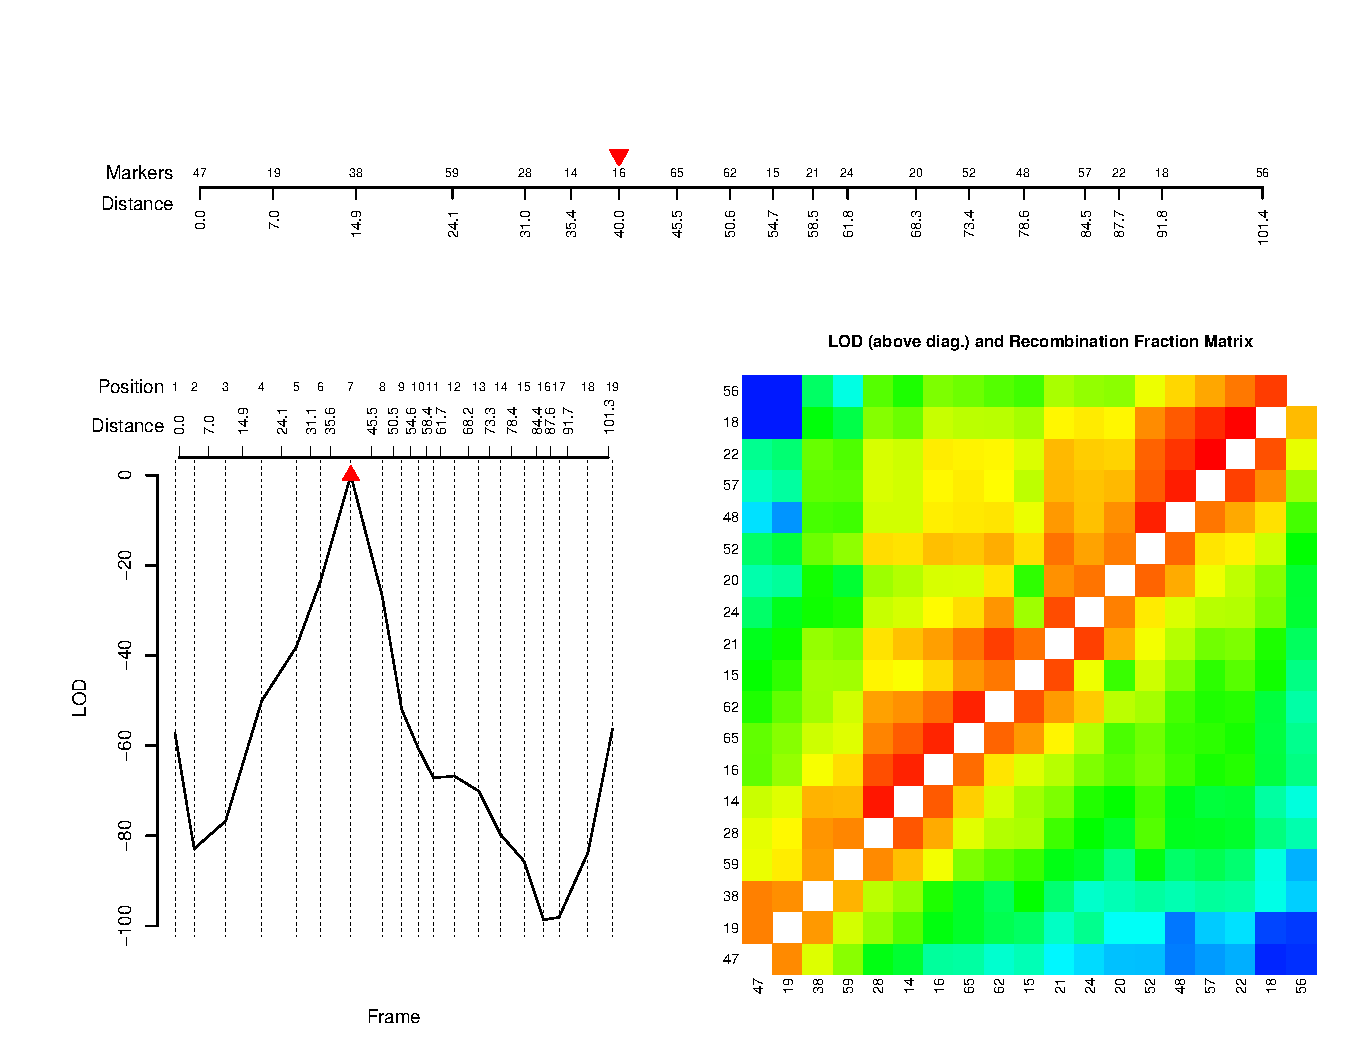
\includegraphics[width=.8\textwidth]{figures/tutorial}
  
 
  
  \vspace{.8in}
  
  {\renewcommand{\baselinestretch}{3}
    Department of Genetics\\
    Escola Superior de Agricultura ``Luiz de Queiroz'' (ESALQ)\\
    Universidade de S\~ao Paulo (USP) - Brazil\\
    E-mail: augusto.garcia@usp.br
  }

\vspace{0.5cm}
\noindent \textsuperscript{*}corresponding author\\
\today
 \end{titlepage}

\tableofcontents
\newpage


\section{Overview}
\label{overview}
(The full version of this tutorial, with all \textsl{OneMap} outputs,
can be found at \url{http://statgen.esalq.usp.br/Tutorial_Onemap_complete_version.pdf})

{\sl OneMap} is an environment for constructing linkage maps in several experimental crosses, including outcrossing (full-sib families derived from two non-homozygous parents), RILs, F$_2$ and backcrosses. It is implemented as a package to be used under the freely distributed R software, which is a language and environment for statistical computing (\url{www.r-project.org}). It is designed to be fully integrated with R/qtl package (Broman et al., 2008) and Windows QTL Cartographer (Wang et al., 2010) in order to do QTL mapping.

Wu et al. (2002a) proposed a methodology to construct genetic maps in outcrossing species, which allows the analysis of a mixed set of different marker types containing various segregation patterns. Also, it allows the simultaneous estimation of linkage and linkage phases between markers, and was successfully applied in the analysis of sugarcane (Garcia et al., 2006; Oliveira et al., 2007) and {\it Passiflora} (Oliveira et al., 2008) data sets. Actually, the analysis of these data sets motivated the implementation of the first release of {\sl OneMap} (Margarido et al., 2007). 

After extensively testing the software, we noticed that the construction of linkage maps could be greatly enhanced with the use of multipoint likelihood through Hidden Markov Models (HMM). Jiang and Zeng (1997) explained in detail this methodology, emphasizing its advantages and limitations for populations derived from inbred lines. Merging the ideas of Wu et al. (2002a) and the HMM framework, as done by Wu et al. (2002b), we then developed version 1.0-0 of {\sl OneMap}, which could order markers using HMM-based algorithms for outcrossing species, in a similar way as implemented in MAPMAKER/EXP (Lander et al., 1987). We verified the great advantages of the new procedure through extensive simulations.

In version 2.0-0, we included several major modifications to take advantage of the fact that some segregation patterns that occur in outcrossing populations can also occur in populations derived from inbred lines (i.e. RILs, F$_2$ and backcrosses). For example, a marker that segregates in $1:2:1$ fashion in outcrossing context can be viewed as a co-dominant marker in F$_2$ populations. The main difference is that, for the later, there is no need to estimate linkage phases. Using these ideas, we adapted {\sl OneMap} to also construct genetic maps in RILs, F$_2$ and backcross populations, taking advantage of {\sl OneMap} facilities. Moreover, we also implemented three new ordination algorithms besides the ones included in version 1.0-0: Rapid Chain Delineation - RCD (Doerge, 1996) and TRY (Lander et al., 1987). They are Seriation - SER (Buetow and Chakravarti, 1987), recombination counting and ordering - RECORD (Van Os et al., 2005) and unidirectional growth - UG (Tan and Fu, 2006). They can be used for all experimental crosses included in {\sl OneMap}, and can be chosen to give the best result for any situation faced by the user (Mollinari et al., 2009) 

{\sl OneMap} is available as source code for Windows\texttrademark \ and Unix systems. It is released under the GNU General Public License, is open-source and the code can be changed freely. It comes with no warranty. 

Although no advanced knowledge in R is required to use {\sl OneMap}, in Section \ref{introductiontor} we present a short introduction to R software, where we address the basic knowledge required to start using {\sl OneMap}. People with some knowledge of R could just skip this part. In Section \ref{introonemap}, information about  {\sl OneMap} installation is provided. In Section \ref{outcrossing}, we show the usage of {\sl OneMap} functions for outcrossing (non-inbred) populations. In Section \ref{f2} we do the same for F$_2$ populations, which can also be applied to backcrosses and RILs. All sections could be read independently. 

\subsection{Citation}

\parshape2 0pt \linewidth 0.8cm 16.2cm
Margarido, G.R.A., Souza, A.P. and Garcia, A.A.F. OneMap: software for genetic mapping in outcrossing species. {\bf {\it Hereditas}} 144: 78-79, 2007.

\section{Introduction to R}
\label{introductiontor}

R is a language and environment for statistical computing and graphics. To download R, please visit the Comprehensive R Archive Network (\url{cran.r-project.org}). Although we prefer and recommend the Linux version, in this tutorial, it is assumed that the user is running Windows\texttrademark. Users of R under Linux or Mac\textsuperscript{\textregistered} OS should have no difficult in following this tutorial. 

After installing R, you can launch it by double-clicking the R icon created on your desktop during the installation process. You will see a window with the R Console (Figure \ref{rconsole}).

\begin{figure}[ht!]
  \centering
  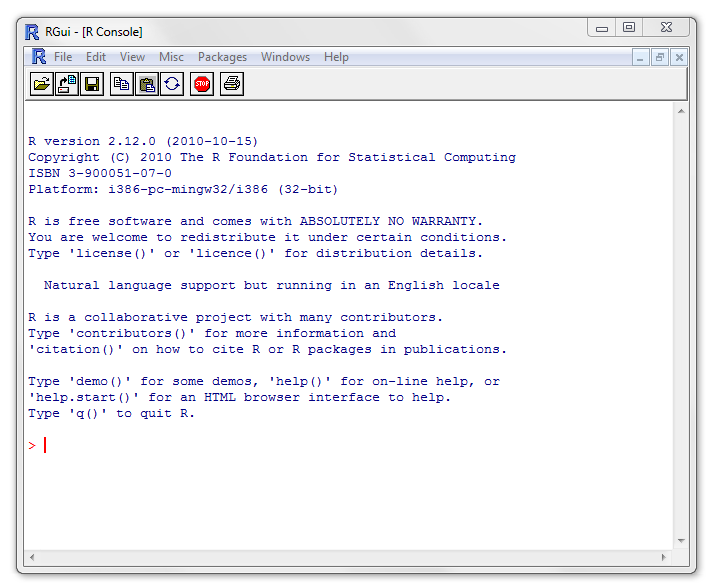
\includegraphics[width=.7\textwidth]{figures/rconsole.png}
  \caption{The R Console.}
   \label{rconsole}
\end{figure}

\subsection{Getting started}

In Figure \ref{rconsole}, you can see a {\it greater than} sign (``>''), which means that R is waiting for a command. We call this {\it prompt}. Let us start with a simple example adding two numbers. Type ``2+3'' at the prompt then type the {\tt Enter} key:
\begin{Schunk}
\begin{Sinput}
> 2+3
\end{Sinput}
\end{Schunk}
You can see the result directly on the screen. You can store this result into a variable for future use, applying the assignment operator {\tt <-} ({\it less than} sign and {\it minus}, altogether):
\begin{Schunk}
\begin{Sinput}
> x<-2+3
\end{Sinput}
\end{Schunk}
The result of the calculation was stored into the variable {\tt x}. You can access this result typing ``x'' at the prompt:
\begin{Schunk}
\begin{Sinput}
> x
\end{Sinput}
\end{Schunk}
You can also use the variable {\tt x} into another calculation, for example:
\begin{Schunk}
\begin{Sinput}
> x+4
\end{Sinput}
\end{Schunk}

\subsection{Functions}
\label{functions}
Another fundamental aspect in R is the usage of {\it functions}. A function is a predefined routine used to do specific calculations. For example, to calculate the natural logarithm of $6.7$, we can use the function {\tt log}:
\begin{Schunk}
\begin{Sinput}
> log(6.7)
\end{Sinput}
\end{Schunk}
The function {\tt log} contains a group of internal procedures to calculate the natural logarithm of a positive real number. The input values of a function are called {\it arguments}. In previous example, we provided only one argument to the function ($6.7$). Sometimes a function has more than one argument. For example, to obtain the logarithm of $6.7$ to base $4$, you can use:
\begin{Schunk}
\begin{Sinput}
> log(6.7,base=4)
\end{Sinput}
\end{Schunk}
It is possible to calculate the natural logarithm of a set of numbers by defining a vector and using it as the first argument of the function {\tt log}. To do so we use the function {\tt c}, that {\it combines} a set of values into a vector. Thus, to calculate the logarithm of the numbers 6.7, 3.2, 5.4, 8.1, 4.9, 9.7 and 2.5, we can use:
\begin{Schunk}
\begin{Sinput}
> y<-c(6.7, 3.2, 5.4, 8.1, 4.9, 9.7, 2.5)
> log(y)
\end{Sinput}
\end{Schunk}

\subsection{Getting help}

Every R function has a help page which can be accessed using a question mark before the name of the function. For example, to get help on function {\tt log}, you would type:

\begin{Schunk}
\begin{Sinput}
> ?log
\end{Sinput}
\end{Schunk}

This command will open a help page in the default web browser of your system. The help page contains some important information about the function such its syntax, its arguments and some usage examples.  

\subsection{Packages} 
\label{packages}
Although R has a huge amount of internal functions, for doing more specific computations, like constructing genetic linkage maps, it is necessary to use complementary functions. These functions can be obtained by installing a {\it package}. A package is a collection of related functions, help files and example data files that have been bundled together (Adler, 2010). 

For example, let us assume you need to convert a set of recombination fractions into centimorgan distance using the Kosambi function. One possible way to do that, is to use the basic R functions to calculate the distances. Another way is use the {\it OneMap} package. To install {\it OneMap} you can type:

\begin{Schunk}
\begin{Sinput}
> install.packages("onemap")
\end{Sinput}
\end{Schunk}

You also can use the console menus: {\it Packages} $ \rightarrow $ {\it Install package(s)}. After clicking, a box will pop-up asking you to choose the CRAN mirror. Choose the location nearest to you. Then, another box will pop-up asking you to choose the package you want to install. Select {\tt onemap} then click {\it OK}. The package will be automatically installed on your computer. Returning to the console, you need to load {\it OneMap} by typing:

\begin{Schunk}
\begin{Sinput}
> library("onemap")
\end{Sinput}
\end{Schunk}

Let us enter some recombination fractions, for example, 0.01, 0.12, 0.05, 0.11, 0.21, 0.07, and save it into a variable called {\tt rf}:

\begin{Schunk}
\begin{Sinput}
> rf<-c(0.01, 0.12, 0.05, 0.11, 0.21, 0.07)
\end{Sinput}
\end{Schunk}

Now, let us use the function {\tt kosambi}, which belongs to {\it OneMap} package, to do the calculation:

\begin{Schunk}
\begin{Sinput}
> kosambi(rf)
\end{Sinput}
\end{Schunk}

You can also obtain help on the function {\tt kosambi} using the question mark in the same way it was done with function {\tt log}:

\begin{Schunk}
\begin{Sinput}
> ?kosambi
\end{Sinput}
\end{Schunk}

\subsection{Importing and exporting data}
\label{import} 
So far, we entered the variables in R by typing them directly into the console. However, in real situations we usually {\it read} these values from a file or a data bank. To exemplify this procedure, copy and paste the following table into a text editor (for example, {\it notepad}) and save it to a file called {\tt test.txt} into your {\it working directory} (such as {\it My Documents}).

\begin{footnotesize}
\begin{verbatim}
        x       y
     2.13    4.50
     4.48    1.98
    10.95    9.29
    10.03   16.25
    12.72   27.38
    24.63   22.60
    22.57   36.87
    29.78   31.73
    19.54   10.42
     7.86   14.68
    11.75    8.68
    23.71   37.39
\end{verbatim}
\end{footnotesize}

To read these data in R, first, we have to set the working directory using the function {\tt setwd}.  For example, if {\tt"C:/Users/mmollina/Documents"} is the full path to {\it My Documents} directory, one should use:

\begin{Schunk}
\begin{Sinput}
> setwd("C:/Users/mmollina/Documents")
\end{Sinput}
\end{Schunk}

Every time you inform paths, directories or files you have to use double quotes (`` ''), which indicates a string of characters instead of a variable. You also can use the console menus to set the working directory: {\it File} $ \rightarrow $ {\it Change Dir...}. From here, every object will be read or saved to this directory.

Now let us read the file {\tt test.txt} into R and store it in a variable called {\tt dat} using the function {\tt read.table}. The first argument is the name of the file. The second indicates if the file contains a header, i. e.  if the first line of the file contains the names of the variables:

\begin{Schunk}
\begin{Sinput}
> (dat<-read.table(file="test.txt", header=TRUE))
\end{Sinput}
\end{Schunk}


Notice that the whole command line is limited by parenthesis. This indicates to R to show the results at the same time you store then into a variable. One could type the command without parenthesis and then type {\tt dat} at the prompt, to produce the same result. Inspecting the object {\tt dat} you can see a table with 12 rows and two columns. The names of the columns are {\tt x} and {\tt y}. We can access the variables in columns using the dollar sign followed by the column name:

\begin{Schunk}
\begin{Sinput}
> dat$x
> dat$y 
\end{Sinput}
\end{Schunk}

It is also possible to use a function called {\tt summary} to extract some information about the object {\tt dat} or about each one of the columns separately:: 

\begin{Schunk}
\begin{Sinput}
> summary(dat)
> summary(dat$x)
> summary(dat$y)
\end{Sinput}
\end{Schunk}

The function {\tt summary} provides some basic statistics about the variables in the dataset. If you want to export these information to a file you can use the function {\tt write.table}:

\begin{Schunk}
\begin{Sinput}
> write.table(x=summary(dat), file="test_sum.txt", quote=FALSE)
\end{Sinput}
\end{Schunk}

The first argument is the output of the {\tt summary} function. Note that is possible to use a function as an argument of another one. The second argument is the name of the file in which the summary is going to be written. Notice that the file will be written in the {\it working directory}, previously set. The third argument eliminates double quotes from the output file. After running the command, you can look for the file {\tt test\_sum.txt} in the {\it working directory}.
 
\subsection{Classes and methods}

In R, every object belongs to a {\it class}. For example, the object {\tt dat} belongs to a class called {\tt data.frame}. We can obtain this information using the function {\tt class}:

\begin{Schunk}
\begin{Sinput}
> class(dat)
\end{Sinput}
\end{Schunk}

When we use the function {\tt summary}, it recognizes the class of the {\tt dat} and applies a specific procedure to the {\tt data.frame} class, which in this case involves the computation of some descriptive statistics. This procedure is called {\it method}. However, another classes of objects can be used as arguments to function {\tt summary} and the result will be different. For example, let us adjust a linear model using column {\tt y} as the dependent variable and column {\tt x} as independent. This can be done with the function {\tt lm()}:

\begin{Schunk}
\begin{Sinput}
> ft.mod<-lm(dat$y~dat$x)
> ft.mod
\end{Sinput}
\end{Schunk}

Function {\tt lm} is used to fit linear models and, by default, returns just a formula and the coefficients of the linear regression. Object {\tt ft.mod} is of class {\tt lm}:

\begin{Schunk}
\begin{Sinput}
> class(ft.mod)
\end{Sinput}
\end{Schunk}

To obtain more information about the fitted model, we can use the function {\tt summary}:

\begin{Schunk}
\begin{Sinput}
> summary(ft.mod)
\end{Sinput}
\end{Schunk}

In this case, the function {\tt summary} recognizes {\tt lm.fit} as an object of class {\tt lm} and applies a method which shows information about the fitted model such as distribution of the residuals, regression coefficients, t-tests, and the coefficient of determination ($r^2$), etc (significance stars not shown). Thus, it is possible to use the same function in different classes of object to obtain different results. This concept is very important in {\it OneMap}. For example, depending on the class of the dataset, which can be {\tt outcross}, {\tt f2.onemap}, {\tt bc.onemap}, {\tt riself.onemap} and {\tt risib.onemap}, a certain set of procedures will be applied.


\subsection{Saving a Workspace}
\label{savework} 

You can save your analysis using the function {\tt save.image}. For example, if you want to save your analysis in a file called {\tt myworkspace.RData}, you should use:

\begin{Schunk}
\begin{Sinput}
> save.image("myworkspace.RData")
\end{Sinput}
\end{Schunk}

You can also use the console menus: {\it File} $ \rightarrow $ {\it Save Workspace}. Now, you can load your analysis into R, using the function {\tt load}:

\begin{Schunk}
\begin{Sinput}
> load("myworkspace.RData")
\end{Sinput}
\end{Schunk}

This is useful if you want to stop one session and continuing on the following day, etc.

\section{Installation and Introduction to OneMap}
\label{introonemap}
{\sl OneMap} can be installed by opening R and typing the command

\begin{Schunk}
\begin{Sinput}
> install.packages("onemap")
\end{Sinput}
\end{Schunk}

You also can use the console menus: {\it Packages} $ \rightarrow $ {\it Install package(s)}. After clicking, a box will pop-up asking you to choose the CRAN mirror. Choose the location nearest to you. Then, another box will pop-up asking you to choose the package you want to install. Select {\tt onemap} then click {\it OK}. The package will be automatically installed on your computer. 

{\sl OneMap} can also be installed by downloading the appropriate files directly at the CRAN web site and following the instructions given in the section ``6.3 Installing Packages'' of the ``R Installation and Administration'' manual (\url{http://cran.r-project.org/doc/manuals/R-admin.pdf}).

{\sl OneMap} is comprised by set of functions (listed on Table \ref{commandtable}). There are other functions used internally by the software. However, you do not need to use them directly.

\begin{table}[!ht]
  \centering
  \small
  \caption{{\sl OneMap} functions}
  \label{commandtable}
  \begin{tabular}{lll}
    \hline\hline
    {\bf Function type}    & {\bf Function name} & {\bf Function description} \\
    \hline
    {\bf Input}             & read.onemap  & Read data from an outcross \\
                               & read.mapmaker  & Read data from a Mapmaker raw file \\
    \hline
    {\bf Data manipulation} & make.seq       & Creates a sequence of markers based on objects of \\
                               &                & other types \\
                               & marker.type    & Informs the segregation type of genetic markers \\
                               & add.marker     & Adds markers to a sequence\\
                               & drop.marker    & Drops markers from a sequence\\
    \hline
    {\bf Genetic mapping}   & rf.2pts        & Estimates recombination fractions (two points) \\
                               & group          & Assigns markers to linkage groups \\
                               & set.map.fun    & Defines the default mapping function\\
                               & rcd            & Orders markers in a sequence using RCD algorithm \\
                               & seriation      & Orders markers in a sequence using SERIATION algorithm \\
                               & record         & Orders markers in a sequence using RECORD algorithm \\
                               & ug             & Orders markers in a sequence using UG algorithm \\
                               & compare        & Compares all possible orders of markers in a sequence \\
                               & try_seq        & Tries to map a marker into a given linkage group \\
                               & order.seq      & Automates map construction through ``compare'' and \\
                               &                & ``try_seq'' functions \\
                               & ripple_seq     & Compares alternative orders for a map and displays \\ 
                               &                & the plausible ones \\
                               & map            & Constructs a multipoint linkage map for a sequence \\
                               &                & in a given order \\
                               & rf.graph.table & Plots a pairwise recombination fraction and LOD \\  
                               &                & matrix using a color scale. \\
                               & draw.map       & Draws a genetic map \\                     
     \hline
    {\bf Output}            & write.map      & Writes a genetic map to a file to be used in other \\
                               &                & softwares (only for backcrosses, F$_2$ and RILs) \\
    \hline
    {\bf Defunct}          & def.rf.3pts     & Estimates recombination fractions (three points method) \\
    \hline\hline
  \end{tabular}
\end{table}
   
After {\sl OneMap} is installed, you can load it with

\begin{Schunk}
\begin{Sinput}
> library(onemap)
\end{Sinput}
\end{Schunk}

A list of packages and datasets that are available on your computer can be obtained with

\begin{Schunk}
\begin{Sinput}
> library()
> data()
\end{Sinput}
\end{Schunk}

\section{Outcrossing  populations}
\label{outcrossing}
The following example is intended to show the usage of {\sl OneMap} functions for linkage mapping in {\bf outcrossing} (non-inbred) species. With basic knowledge of R syntax, one should have no big problems using it. If you are not familiar with R software, we recommend reading Section \ref{introductiontor}. It is assumed that the user is running Windows\texttrademark. Hopefully these examples will be clear enough to help any user to understand its functionality and start using it.

\begin{enumerate}
\item Start R by double-clicking its icon.

\item Load {\sl OneMap}, after installing it:
\begin{Schunk}
\begin{Sinput}
> library(onemap)
\end{Sinput}
\end{Schunk}

\item To save your project anytime, type:
\begin{Schunk}
\begin{Sinput}
> save.image("C:/.../yourfile.RData")
\end{Sinput}
\end{Schunk}
or access the toolbar File $\to$ Save Workspace.
\end{enumerate}


\subsection{Creating the data file}
This step might be quite difficult, since the data file is not very simple and many errors can occur while reading it. The input file format is similar to that used by MAPMAKER/EXP (Lander et al., 1987), so experienced users of genetic analysis software should be already familiar with it.

Basically, the input file is a text file, where the first line indicates the number of individuals and the number of markers. Then, the genotype information is included separately for each marker. The character ``*'' indicates the beginning of information input for a new marker, followed by the marker name. Next, there is a code indicating the marker type, according to Wu's et al. (2002a) notation (Table \ref{segregout})

\vspace{.5cm}


\begin{table}[!ht]
  \centering
  \scriptsize
  \caption{Notation used to identify markers and genotypes}
  \label{segregout}
  \begin{tabular}{c c r r c l c r c l c c c}
    \hline \hline
          &      &     & \multicolumn {7}{p{3cm}}{Parent}	& &\multicolumn {2}{p{3cm}}{Offspring}	\\
        \cline{4-10} \cline{12-13}
          &      & crosstype & \multicolumn {3}{p{.4cm}}{Cross}& & \multicolumn {3}{p{.4cm}} {Observed bands} &  & Observed bands	& Segregation	\\
        \hline
        A &     & 1 & $ab $ & $\times$ & $ cd$  & & $ab $ & $\times$ & $ cd$  & & $ac, ad, bc, bd$ & 1:1:1:1 \\
          &     & 2 & $ab $ & $\times$ & $ ac$  & & $ab $ & $\times$ & $ ac$  & & $ a, ac, ba, bc$ & 1:1:1:1 \\
          &     & 3 & $ab $ & $\times$ & $ co$  & & $ab $ & $\times$ & $ c$   & & $ac,  a, bc,  b$ & 1:1:1:1 \\
          &     & 4 & $ao $ & $\times$ & $ bo$  & & $a $  & $\times$ & $ b$   & & $ab,  a,  b,  o$ & 1:1:1:1 \\[1.2ex]
        B &B$_1$& 5 & $ab $ & $\times$ & $ ao$  & & $ab $ & $\times$ & $ a$   & & $ab, 2a,  b$     & 1:2:1\\[1.2ex]
          &B$_2$& 6 & $ao $ & $\times$ & $ ab$  & & $a $  & $\times$ & $ ab$  & & $ab, 2a,  b$     & 1:2:1\\[1.2ex]
          &B$_3$& 7 & $ab $ & $\times$ & $ ab$  & & $ab $ & $\times$ & $ ab$  & & $a, 2ab,  b$     & 1:2:1\\[1.2ex]
        C &     & 8 & $ao $ & $\times$ & $ ao$  & & $a $  & $\times$ & $ a$   & & $3a, o$          & 3:1\\[1.2ex]
        D &D$_1$& 9 & $ab $ & $\times$ & $ cc$  & & $ab $ & $\times$ & $ c$   & & $ac, bc$         & 1:1 \\
          &     & 10& $ab $ & $\times$ & $ aa$  & & $ab $ & $\times$ & $ a$   & & $a, ab$         & 1:1 \\
          &     & 11& $ab $ & $\times$ & $ oo$  & & $ab $ & $\times$ & $ o$   & & $a, b$           & 1:1 \\
          &     & 12& $bo $ & $\times$ & $ aa$  & & $b $  & $\times$ & $  a$  & & $ab, a$          & 1:1 \\
          &     & 13& $ao $ & $\times$ & $ oo$  & & $a $  & $\times$ & $  o$  & & $a, o$           & 1:1 \\[1.2ex]
          &D$_2$& 14& $cc $ & $\times$ & $ ab$  & & $c  $ & $\times$ & $ ab$  & & $ac, bc$         & 1:1 \\
          &     & 15& $aa $ & $\times$ & $ ab$  & & $a $  & $\times$ & $ ab$  & & $a, ab$          & 1:1 \\
          &     & 16& $oo $ & $\times$ & $ ab$  & & $o $  & $\times$ & $ ab$  & & $a, b$           & 1:1 \\
          &     & 17& $aa $ & $\times$ & $ bo$  & & $a  $ & $\times$ & $ b$   & & $ab, a$          & 1:1 \\
          &     & 18& $oo $ & $\times$ & $ ao$  & & $o $  & $\times$ & $  a$  & & $a, o$           & 1:1 \\
        \hline \hline
      \end{tabular}
\end{table}

\vspace{.5cm}

Actually, it is recommended to check Wu's et al. (2002a) paper before using {\sl OneMap}. Marker types must be one of the following: {\sl A.1, A.2, A.3, A.4, B1.5, B2.6, B3.7, C.8, D1.9, D1.10, D1.11, D1.12, D1.13, D2.14, D2.15, D2.16, D2.17} or {\sl D2.18}, each one corresponding to a row of the table. The letter and the number before the dot indicate the segregation type (i.e., 1:1:1:1, 1:2:1, 3:1 or 1:1), while the number after the dot indicates the observed bands in the offspring. The paper cited above gives details with respect to marker types; we will not discuss them here, but it is easy to see that each marker is classified based on the band patterns on parents and progeny.

Finally, after each marker name, comes the genotype data for the segregating population. The coding for marker genotypes used by {\sl OneMap} is also the same one proposed by Wu et al. (2002a) and the possible values vary according to the specific marker type. Missing data are indicated with the character ``-'' (minus sign) and a comma separates the information for each individual.

Here is an example of such file for 10 individuals and 5 markers:

\begin{verbatim}
   10 5
   *M1 B3.7        ab,ab,-,ab,b,ab,ab,-,ab,b
   *M2 D2.18       o,-,a,a,-,o,a,-,o,o
   *M3 D1.13       o,a,a,o,o,-,a,o,a,o
   *M4 A.4         ab,b,-,ab,a,b,ab,b,-,a
   *M5 D2.18       a,a,o,-,o,o,a,o,o,o
\end{verbatim}

Notice that once the marker type is identified, no variations of symbols presented on the table for the ``observed bands'' is allowed. For example, for {\sl A.1}, only {\tt ac}, {\tt ad}, {\tt bc} and {\tt bd} genotypes are expected (plus missing values). We notice that this is a common mistake made by users, so be careful. 

The input file must be saved in text format, with extensions like ``.txt''. It is a good idea to open the text file called ``example.out.raw'' (available with {\sl OneMap} and saved in the directory you installed it to see how this file should be. You can see where {\sl OneMap} is installed using the command 

\begin{Schunk}
\begin{Sinput}
> system.file(package="onemap")
\end{Sinput}
\end{Schunk}

\subsection{Importing data}
\begin{enumerate}
\item Once the input file is created, data can be loaded and saved into an R object. The function used to import data is named {\tt read.onemap}. Its usage is quite simple:
\begin{Schunk}
\begin{Sinput}
> example.out<- read.onemap("C:/workingdirectory","example.out.raw")
\end{Sinput}
\end{Schunk}
The first argument is the directory where the input file is located, so modify it accordingly.  The second one is the data file name. In this example, an object named {\tt example.out} was created. If you leave the argument {\tt dir} blank, the file will be read from your {\it working directory}. To set a working directory, see Section \ref{import}.

\item You can change the working directory in R using function {\tt setwd()} or in the toolbar clicking File $\to$ Change dir. If you set your working directory to the one containing the input file, you can just type:
\begin{Schunk}
\begin{Sinput}
> example.out<- read.onemap(file="example.out.raw")
\end{Sinput}
\end{Schunk}

If no error has occurred, a message will display some basic information about the data, such as number of individuals and number of markers:

\item Because this particular data set is distributed along with the package, as an alternative you can load it typing
\begin{Schunk}
\begin{Sinput}
> data(example.out)
\end{Sinput}
\end{Schunk}

\item Loading the data creates an object of class {\tt outcross}, which will further be used in the analysis. R command {\tt print} recognizes objects of this class. Thus, if you type
\begin{Schunk}
\begin{Sinput}
> example.out
\end{Sinput}
\end{Schunk}

you will see some information about the object.

\end{enumerate}

\subsection{Estimating two-point recombination fractions}
\begin{enumerate}
\item To start the analysis, the first step is estimating the recombination fraction between all pairs of markers, using two-point tests:
\begin{Schunk}
\begin{Sinput}
> twopts <- rf.2pts(example.out)
\end{Sinput}
\end{Schunk}
The function {\tt rf.2pts} uses as default values of LOD Score 3 and maximum recombination fraction 0.50.

\item Different values for the criteria can be chosen using:
\begin{Schunk}
\begin{Sinput}
> twopts <- rf.2pts(example.out, LOD=3, max.rf=0.4)
\end{Sinput}
\end{Schunk}

\item Although two-point tests were implemented in C language, which is much faster than R, this step can take quite some time, depending on the number of markers involved and their segregation type, since all combinations will be estimated and tested. Besides, the results use a lot of memory and a rather powerful computer is needed. For example, the analysis of a real data set with 1741 markers (segregating 3:1 and 1:1) took 2.8 hours, running under Windows\texttrademark \ on a Pentium\textsuperscript{\textregistered} 4 CPU 3.00 GHz with 1 GB RAM memory.

\item When the two-point analysis is finished, an object of class {\tt rf.2pts} is created. Typing
\begin{Schunk}
\begin{Sinput}
> twopts
\end{Sinput}
\end{Schunk}
will show a message with the criteria used in the analysis and some other information:


\item If you want to see the results for given markers, say {\tt M1} and {\tt M3}, the command is:
\begin{Schunk}
\begin{Sinput}
> print(twopts, "M1", "M3")
\end{Sinput}
\end{Schunk}

Each line corresponds to a possible linkage phase. 1 denotes coupling phase in both parents (CC), 2 and 3 denote coupling phase in parent 1 and 2, respectively, and repulsion in the other (CR and RC), and 4 denotes repulsion phase in both parents (RR). Theta is the maximum likelihood estimate of the recombination fraction, with its LOD Scores.

\end{enumerate}

\subsection{Assigning markers to linkage groups}
\begin{enumerate}
\item Once the recombination fractions and linkage phases for all pairs of markers have been estimated and tested, markers can be assigned to linkage groups. To do this, first use the function {\tt make.seq} to create a sequence with the markers you want to assign:
\begin{Schunk}
\begin{Sinput}
> mark.all <- make.seq(twopts, "all")
\end{Sinput}
\end{Schunk}
The function {\tt make.seq} is used to create sequences from objects of several kinds, as will be seen along this tutorial. Here, the object is of class {\tt rf.2pts} and the second argument specifies which markers one wants to use. In this example, the argument {\tt "all"} indicates that all markers will be analyzed. If one wants to use only a subset of markers, say {\tt M1} and {\tt M2}, the option will be {\tt c(1,2)}. These numbers refer to the lines where markers are located on the data file. Since the identification of the markers can be cumbersome, one should use the function {\tt marker type} to see their numbers, names and types:

\begin{Schunk}
\begin{Sinput}
> marker.type(mark.all)
\end{Sinput}
\end{Schunk}

\item The grouping step is very simple and can be done by using the function {\tt group}:
\begin{Schunk}
\begin{Sinput}
> LGs <- group(mark.all)
\end{Sinput}
\end{Schunk}
For this function, optional arguments are {\tt LOD} and {\tt max.rf}, which define thresholds to be used when assigning markers to linkage groups. If none provided (default), criteria previously defined for the object {\tt twopts} are used.

\item The previous command generates an object of class {\tt group} and the command {\tt print} for such object has two options. If you type:
\begin{Schunk}
\begin{Sinput}
> LGs
\end{Sinput}
\end{Schunk}

you will get detailed information about the groups, i.e., all linkage groups will be printed, displaying the names of markers in each one of them.

However, in case you just want to see some basic information (such as the number of groups, number of linked markers, etc):
\begin{Schunk}
\begin{Sinput}
> print(LGs, detailed=FALSE)
\end{Sinput}
\end{Schunk}

\item You can notice that all markers are linked to some linkage group. If the LOD Score threshold is changed to a higher value, some markers are kept unassigned:
\begin{Schunk}
\begin{Sinput}
> LGs <- group(mark.all, LOD=6)
> LGs
\end{Sinput}
\end{Schunk}

\item Changing back to the previous criteria, now setting the maximum recombination fraction to 0.40:
\begin{Schunk}
\begin{Sinput}
> LGs <- group(mark.all, LOD=3, max.rf=0.4)
> LGs
\end{Sinput}
\end{Schunk}
\end{enumerate}

\subsection{Genetic mapping of linkage group 3}
\label{group3outcrossing}
\begin{enumerate}
\item Once marker assignment to linkage groups is finished, the mapping step can take place. First of all, you must set the mapping function that should be used to display the genetic map through the analysis. You can choose between Kosambi or Haldane mapping functions. To use Haldane, type
\begin{Schunk}
\begin{Sinput}
> set.map.fun(type="haldane")
\end{Sinput}
\end{Schunk}

To use Kosambi
\begin{Schunk}
\begin{Sinput}
> set.map.fun(type="kosambi")
\end{Sinput}
\end{Schunk}

Now, you must define which linkage group will be mapped. In other words, a linkage group must be ``extracted'' from the object of class {\tt group}, in order to be mapped. For simplicity, we will start here with the smallest one, which is linkage group 3. This can be easily done using the following code:
\begin{Schunk}
\begin{Sinput}
> LG3 <- make.seq(LGs, 3)
\end{Sinput}
\end{Schunk}
The first argument ({\tt LGs}) is an object of class {\tt group} and the second is a number indicating which linkage group will be extracted, according to the results stored in object {\tt LGs}. The object {\tt LG3}, generated by function {\tt make.seq}, is of class {\tt sequence}, showing that this function can be used with several types of objects.

\item If you type
\begin{Schunk}
\begin{Sinput}
> LG3
\end{Sinput}
\end{Schunk}
you will see which markers are comprised in the sequence, and also that no parameters have been estimated.

\item To order these markers, one can use a two-point based algorithm such as Seriation (Buetow and Chakravarti, 1987), Rapid Chain Delineation (Doerge, 1996), Recombination Counting and Ordering (Van Os et al., 2005) and Unidirectional Growth (Tan and Fu, 2006):
  
\begin{Schunk}
\begin{Sinput}
> LG3.ser <- seriation(LG3)
> LG3.rcd <- rcd(LG3)
> LG3.rec <- record(LG3)
> LG3.ug  <- ug(LG3)
\end{Sinput}
\end{Schunk}

In this case, all algorithms provided the same results (results not showed).

\item To order by comparing all possible orders (exhaustive search), the function {\tt compare} can be used:
\begin{Schunk}
\begin{Sinput}
> LG3.comp <- compare(LG3)
\end{Sinput}
\end{Schunk}

This order step can take some time, depending on marker types in the linkage group. In the example, {\tt LG3} contains one marker of type D1 and one of type D2, besides one marker segregating in 3:1 fashion (type C). Thus, although the number of possible orders is relatively small (60), for each order there are various possible combinations of linkage phases. Also, the convergence of the EM algorithm takes considerably more time, since markers of type C are not very informative. 

The first argument to {\tt compare} function is an object of class {\tt sequence} (the extracted group {\tt LG3}), and the object generated by this function is of class {\tt compare}.

\item To see the results of the previous step, type
\begin{Schunk}
\begin{Sinput}
> LG3.comp
\end{Sinput}
\end{Schunk}

Remember that for outcrossing populations, one needs to estimate marker order and also linkage phases between markers for a given order. However, since two point analysis also provided information about linkage phases, this information was taken into consideration in the {\tt compare} function, reducing the number of combinations to be evaluated. If at least one linkage phase has LOD equals to 0.005 in the two point analysis, we assumed that this phase is very unlikely and so do not need to be evaluated in the multipoint procedure used by compare. We did extensive simulations that showed that this is a good procedure. 

By default, {\it OneMap} stores 50 orders, which may or may not be unique. The value of {\tt LOD} refers to the overall LOD Score, considering all orders tested. {\tt Nested LOD} refers to LOD Scores \emph{within} a given order, i.e., scores for different combinations of linkage phases for the same marker order.

For example, order 1 has the largest value of log-likelihood and, therefore, its LOD Score is zero for a given combination of linkage phases (CC, CC, RR, RR). For this same order and other linkage phases, LOD Score is -2.43. Analyzing the results for order 2, notice that its highest LOD Score is very close to zero, indicating that this order is also quite plausible. Notice also that {\tt Nested LOD} will always contain at least one zero value, corresponding to the best combination of phases for markers in a given order. Due to the information provided by two-point analysis, not all combinations are tested and that is the reason why the number of Nested LOD is different for each order.

\item Unless one has some biological information, it is a good idea to choose the order with the highest likelihood. The final map can then be obtained with the command
\begin{Schunk}
\begin{Sinput}
> LG3.final <- make.seq(LG3.comp,1,1)
\end{Sinput}
\end{Schunk}

The first argument is the object of class {\tt compare}. The second argument indicates which order is chosen: 1 is for the order with highest likelihood, 2 is for the second best, and so on. The third argument indicates which combination of phases is chosen for a given order: 1 also means the combination with highest likelihood among all combinations of phases (based on Nested LOD).

For simplicity, these values are defaults, so typing
\begin{Schunk}
\begin{Sinput}
> LG3.final <- make.seq(LG3.comp)
\end{Sinput}
\end{Schunk}
will have the same effect.

\item To see the final map type
\begin{Schunk}
\begin{Sinput}
> LG3.final
\end{Sinput}
\end{Schunk}

At the leftmost position, marker names are displayed. {\tt Position} shows the cumulative distance using the Kosambi mapping function. Finally, {\tt Parent 1} and {\tt Parent 2} show the diplotypes of both parents, that is, the manner in which alleles are arranged in the chromosomes, given the estimated linkage phase. Notation is the same as that used by Wu et al. (2002a). Details about how ordering algorithms can be chosen and used are presented by Mollinari et al. (2009). 
\end{enumerate}

\subsection{Genetic mapping of linkage group 2}
\label{group2outcrossing}
 Now let us map the markers in linkage group number 2.
 
\begin{enumerate}
\item Again, ``extract'' that group from the object {\tt LGs}:
\begin{Schunk}
\begin{Sinput}
> LG2 <- make.seq(LGs, 2)
> LG2
\end{Sinput}
\end{Schunk}
Note that there are 10 markers in this group, so it is unfeasible to use the {\tt compare} function with all of them since it will take a very long time to proceed.

\item First, use {\tt rcd} to get a preliminary order estimate:
\begin{Schunk}
\begin{Sinput}
> LG2.rcd <- rcd(LG2)
> LG2.rcd
\end{Sinput}
\end{Schunk}

\item Use the {\tt marker.type} function to check the segregation types of all markers in this group:
\begin{Schunk}
\begin{Sinput}
> marker.type(LG2)
\end{Sinput}
\end{Schunk}

\item Based on their segregation types and distribution on the preliminary map, markers M4, M23, M19, M20 and M24 are the most informative ones (type A is the better, followed by type B). So, let us create a framework of ordered markers using {\tt compare} for the most informative ones: 
\begin{Schunk}
\begin{Sinput}
> LG2.init <- make.seq(twopts,c(4,23,19,20,24))
> LG2.comp <- compare(LG2.init)
\end{Sinput}
\end{Schunk}
\begin{Schunk}
\begin{Sinput}
> LG2.comp
\end{Sinput}
\end{Schunk}
Now, the first argument to {\tt make.seq} is an object of class {\tt rf.2pts}, and the second argument is a vector of integers, specifying which molecular markers will be in the sequence.

\item Select the best order:
\begin{Schunk}
\begin{Sinput}
> LG2.frame <- make.seq(LG2.comp)
\end{Sinput}
\end{Schunk}

\item Next, let us try to map the remaining markers, one at a time. Since there are more markers of type D1 than D2, the latter will be tried later. Starting with {\tt M9}:
\begin{Schunk}
\begin{Sinput}
> LG2.extend <- try_seq(LG2.frame,9)
> LG2.extend
\end{Sinput}
\end{Schunk}

Based on the LOD Scores, marker M9 is probably better located between markers M23 and M24. However, the ``*'' symbol indicates that more than one linkage phase is possible. Detailed results can be seen with

\begin{Schunk}
\begin{Sinput}
> print(LG2.extend,5)
\end{Sinput}
\end{Schunk}

The second argument indicates the position where to place the marker. Note that the first allele arrangement is the most likely one. 

Also, we can obtain some useful diagnostic graphics using the argument {\tt draw.try=TRUE} when using function {\tt try_seq}:

\begin{Schunk}
\begin{Sinput}
> LG2.extend <- try_seq(LG2.frame, 9, draw.try=TRUE)
\end{Sinput}
\end{Schunk}

The top figure represents the new genetic map obtained with the insertion of marker 9  between markers M23 and M24 (most likely one). The left bottom figure represents the frame map  M24 - M23 - M4 - M19 - M20 on x-axis and the LOD Scores of the linkage maps obtained with the insertion of marker 9 at the beginning, between markers and at the end of the frame map. The red triangle indicates the most likely position, where the marker 9 it is supposed to be placed. The right bottom figure is the recombination fraction matrix based on a color scale using the function {\tt rf.graph.table}. See Section \ref{recmat} for details. The diagnostic graphics show an almost monotonic recombination fraction matrix (the values are bigger as their distance from diagonal increases). This pattern is typical of ordered linkage groups. We can see that the position between markers {\tt M23} and {\tt M24} is the most likely one for positioning marker {\tt M9}

\item  Finally, the best order can be obtained with:
\begin{Schunk}
\begin{Sinput}
> LG2.frame <- make.seq(LG2.extend,5,1)
\end{Sinput}
\end{Schunk}
When using {\tt make.seq} with an object of class {\tt try}, the second argument is the position on the map (according to the scale on the right of the output) and the last argument indicates linkage phases (defaults to 1, higher nested LOD).

It should be pointed out that the framework created by the function {\tt compare} with ({\tt M20},   {\tt M4},  {\tt M19},  {\tt M23} and {\tt M24}) could be in reverse order ({\tt M24}, {\tt M23}, {\tt M19}, {\tt M4} and {\tt M20}) and still be the same map. Thus, the positioning of markers by command {\tt try_seq} can be different in your computer. For example, here, marker {\tt M9} was better placed in position 5, however if you obtain a reverse order,  marker {\tt M9} would be better placed in position 2. In both cases the best position is between markers {\tt M24} and {\tt M23}.

Adding other markers, one by one (output not shown):

\begin{Schunk}
\begin{Sinput}
> LG2.extend <- try_seq(LG2.frame,29)
> LG2.frame <- make.seq(LG2.extend,7)
> LG2.extend <- try_seq(LG2.frame,27)
> LG2.frame <- make.seq(LG2.extend,1)
> LG2.extend <- try_seq(LG2.frame, 16)
> LG2.frame <- make.seq(LG2.extend,2)
> LG2.extend <- try_seq(LG2.frame,21)
> LG2.final <- make.seq(LG2.extend,6)
\end{Sinput}
\end{Schunk}

\item The process of adding markers sequentially can be automated with the use of function {\tt order.seq}.
  
\begin{Schunk}
\begin{Sinput}
> LG2.ord <- order.seq(LG2, n.init=5, THRES=3, draw.try=TRUE, wait=1)
\end{Sinput}
\end{Schunk}

Basically, this function automates what the {\tt try_seq} function does, using some pre-defined rules. In the function, {\tt n.init = 5} means that five markers (the most informative ones) will be used in the {\tt compare} step; {\tt THRES = 3} indicates that the {\tt try_seq} step will only add markers to the sequence which can be mapped with LOD Score greater than 3; {\tt draw.try=TRUE} will display a diagnostic graphic for each {\tt try_seq} step; {\tt wait=1} indicates the minimum time interval in seconds to display the diagnostic graphic. 

NOTE: Although very useful, this function can be misleading, specially if there are not many fully informative markers, so use it carefully. Results can vary for each running, of course.

\item Check the final order:
\begin{Schunk}
\begin{Sinput}
> LG2.ord
\end{Sinput}
\end{Schunk}
Note that markers {\tt 21} and {\tt 29} could not be safely mapped to a single position ({\tt LOD Score > THRES} in absolute value). The output displays the ``safe'' order and the most likely positions for markers not mapped, where ``***'' indicates the most likely position and ``*'' corresponds to other plausible positions.

\item To get the safe order (i.e. without markers 21 and 29), use 
\begin{Schunk}
\begin{Sinput}
> LG2.safe <- make.seq(LG2.ord,"safe")
\end{Sinput}
\end{Schunk}
and to get the order with all markers, use
\begin{Schunk}
\begin{Sinput}
> LG2.all <- make.seq(LG2.ord,"force")
> LG2.all
\end{Sinput}
\end{Schunk}
Notice that, for this linkage group, the ``forced'' map obtained with {\tt order.seq} is the same as that obtained with {\tt compare} plus {\tt try_seq}, but \emph{this is not always the case}.

\item The {\tt order.seq} function can also performs two rounds of the {\tt try_seq} algorithms, first using {\tt THRES} and then {\tt THRES - 1} as threshold. This generally results in safe orders with more markers mapped, but may take longer to run. To do this use the {\tt touchdown} options:
\begin{Schunk}
\begin{Sinput}
> LG2.ord <- order.seq(LG2, n.init=5, THRES=3, touchdown=TRUE)
> LG2.ord
\end{Sinput}
\end{Schunk}
For this particular sequence, the {\tt touchdown} step could not map any additional marker, but this depends on the specific dataset.

\item Finally, to check for alternative orders (since we did not use exhaustive search), use the {\tt ripple_seq} function:
\begin{Schunk}
\begin{Sinput}
> ripple_seq(LG2.all, ws=4, LOD=3)
\end{Sinput}
\end{Schunk}

We should do this to any of the orders we found, either using {\tt try_seq} or {\tt order.seq}. Here, we choose {\tt LG2.all} only for didactic purpose. The second argument, {\tt ws = 4}, means that subsets (windows) of four markers will be permutated sequentially ({\tt $4!$} orders for each window), to search for other plausible orders. The {\tt LOD} argument means that only orders with LOD Score smaller than 3 will be printed.

The output shows sequences of four numbers, since {\tt ws = 4}.  They will be followed by an {\tt OK}, if there is no alternative orders with LOD Scores smaller than {\tt LOD = 3} in absolute value, or by a list of alternative orders. On the example, just the last sequence showed an alternative order with LOD smaller than {\tt LOD=3} (2.06, in absolute value). However, the best order was the previous one (LOD=0.00). 

If there was an alternative order most likely than the original, one should check the difference between these orders (and linkage phases) and change it using, for example, the function {\tt drop.marker} (see Section \ref{arbitrary}) and {\tt seq.try} or typing the new order. You can use {\tt \$seq.num} and {\tt \$seq.phases} after the name of the sequence (for example, {\tt LG2.all\$seq.num} and {\tt LG2.all\$seq.phases}) to obtain the original order and linkage phases, make the necessary changes (by copying and paste) and then use the function {\tt map} (see Section \ref{arbitrary}) to reestimate the genetic map for the new order.

Here, the function {\tt ripple_seq} showed that the final order obtained is indeed the best for this linkage group. The map can then be printed using  
    
\begin{Schunk}
\begin{Sinput}
> LG2.all
\end{Sinput}
\end{Schunk}

\end{enumerate}

\subsection{Genetic mapping of linkage group 1}
\begin{enumerate}
\item Finally, linkage group 1 (the largest one) will be analyzed. Extract markers:
\begin{Schunk}
\begin{Sinput}
> LG1 <- make.seq(LGs, 1)
\end{Sinput}
\end{Schunk}

\item Construct the linkage map, by automatic using try algorithm:
\begin{Schunk}
\begin{Sinput}
> LG1.ord <- order.seq(LG1, n.init=6, touchdown=TRUE)
> LG1.ord
\end{Sinput}
\end{Schunk}
Notice that the second round of {\tt try_seq} added markers {\tt M5} and {\tt M25}.

\item Now, get the order with all markers:
\begin{Schunk}
\begin{Sinput}
> (LG1.final <- make.seq(LG1.ord,"force"))
\end{Sinput}
\end{Schunk}

\item Check the final map:
\begin{Schunk}
\begin{Sinput}
> ripple_seq(LG1.final)
\end{Sinput}
\end{Schunk}

No better order was observed.

\item Print it
\begin{Schunk}
\begin{Sinput}
> LG1.final
\end{Sinput}
\end{Schunk}

\item As an option, different algorithms to order markers should be applied: 

\begin{Schunk}
\begin{Sinput}
> LG1.ser <- seriation(LG1)
> LG1.rcd <- rcd(LG1)
> LG1.rec <- record(LG1)
> LG1.ug  <- ug(LG1)
\end{Sinput}
\end{Schunk}

There are some differences between the results. Seriation did not provide good results in this case. See Mollinari et al. (2009) for an evaluation of these methods.
  
\end{enumerate}

\subsection{Map estimation for an arbitrary order}
\label{arbitrary}
\begin{enumerate}
\item If, for any reason, one wants to estimate parameters for a given linkage map (e.g. for other orders on published papers), it is possible to define a sequence and use the {\tt map} function. For example, for markers {\tt M30}, {\tt M12}, {\tt M3}, {\tt M14} and {\tt M2}, in this order, use
  
\begin{Schunk}
\begin{Sinput}
> any.seq <- make.seq(twopts,c(30,12,3,14,2))
> (any.seq.map <- map(any.seq))
\end{Sinput}
\end{Schunk}
This is a subset of the first linkage group. When used this way, {\tt map} function searches for the best combination of phases between markers and print the results.

\item Furthermore, a sequence can also have user-defined linkage phases. The next example shows (incorrect) phases used for the same order of markers:
\begin{Schunk}
\begin{Sinput}
> any.seq <- make.seq(twopts,c(30,12,3,14,2),phase=c(4,1,4,3))
> (any.seq.map <- map(any.seq))
\end{Sinput}
\end{Schunk}

\item If one needs to add or drop markers from a predefined sequence, functions {\tt add.marker} and {\tt drop.marker} can be used. For example, to add markers 4 to 8 to {\tt any.seq}
\begin{Schunk}
\begin{Sinput}
> (any.seq <- add.marker(any.seq, 4:8))
\end{Sinput}
\end{Schunk}

Removing markers 3, 4, 5, 12 and 30 from {\tt any.seq}: 
\begin{Schunk}
\begin{Sinput}
> (any.seq <- drop.marker(any.seq, c(3,4,5,12,30)))
\end{Sinput}
\end{Schunk}
\end{enumerate}

After that, the map needs to be re-estimated.

\subsection{Plotting the recombination fraction matrix}
\label{recmat}

For a given sequence, it is possible to plot the recombination fraction matrix and LOD Scores based on a color scale using the function {\tt rf.graph.table}. This matrix can be useful to make some diagnostics about the map. 
  
\begin{enumerate}
\item For example, using the function {\tt group} with {\tt LOD=2.5}:

\begin{Schunk}
\begin{Sinput}
> (LGs <- group(mark.all, LOD=2.5))
\end{Sinput}
\end{Schunk}

Due to the small value used for the LOD Score (2.5, not adequate and resulting in false positives), markers from different groups were placed together.

\item Ordering markers (results not shown):

\begin{Schunk}
\begin{Sinput}
> LG.err<-make.seq(LGs, 2)
> LG.err.ord<-order.seq(LG.err)
\end{Sinput}
\end{Schunk}

The map using option ``force'':

\begin{Schunk}
\begin{Sinput}
> (LG.err.map<-make.seq(LG.err.ord, "force"))
\end{Sinput}
\end{Schunk}


\item A careful examination of the results shows that there are problems on the map. This can be done by plotting the recombination fraction matrix:

\begin{Schunk}
\begin{Sinput}
> rf.graph.table(LG.err.map)
\end{Sinput}
\end{Schunk}



The recombination fractions are plotted below the diagonal and the LOD Scores are plotted above the diagonal. The color scale varies from red (small distances or big LODs) to dark blue. This color scale follows the ``rainbow'' color palette with {\tt start} argument equals to 0 and {\tt end} argument equals to 0.65. White cells indicate for combinations of markers whose recombination fractions cannot be estimated (D$_1$ and D$_2$). 

Clicking on the cell corresponding to two markers (off secondary diagonal), you can see some information about them. For example, clicking on the cell corresponding to markers {\tt M4} and {\tt M19} you can see their names, types ({\tt A.4} and {\tt B1.5}), recombination fraction ({\tt rf=0.02281}) and LOD Scores for each possible linkage phase. Clicking in a cell on the diagonal, some information about the corresponding marker is shown, including percent of missing data. We think this is quite useful in helping to interpret the results. 

Looking at the matrix, it is possible to see two groups: one with markers from {\tt LG2} ({\tt M27},  {\tt M16}, {\tt M20}, {\tt M4}, {\tt M19}, {\tt M21}, {\tt M23}, {\tt M9}, {\tt M24}, and {\tt M29}) and other with markers from {\tt LG3} ({\tt M22}, {\tt M7}, {\tt M18}, {\tt M8} and {\tt M13}). There is a gap between markers {\tt M22} and {\tt M29} ({\tt rf=0.4594}). At this position, the group should be divided, that is, a higher LOD Score should be used.  Notice that these two groups were placed together due to a false linkage (false positive) detected between markers {\tt M4} and {\tt M22} (LOD Score 2.9) due to the fact of not using appropriated LOD threshold (more conservative value). 

The {\tt rf.graph.table} can also be used to check the order of markers based on the monotonicity of the matrix, i.e. as we get away from the secondary diagonal, the recombination fraction values should increase. For another example of function {\tt rf.graph.table}, see Section \ref{recmat2}.

\end{enumerate}

\subsection{Drawing the genetic map}

\begin{enumerate}

  \item Once all linkage groups were obtained, we can draw a simple map using the function {\tt draw.map}. We can draw a genetic map for all linkage groups:

\begin{Schunk}
\begin{Sinput}
> maps<-list(LG1.final, LG2.final, LG3.final)
> draw.map(maps, names= TRUE, grid=TRUE, cex.mrk=0.7)
\end{Sinput}
\end{Schunk}

\item For a specific linkage group:

\begin{Schunk}
\begin{Sinput}
> draw.map(LG1.final, names= TRUE, grid=TRUE, cex.mrk=0.7)
\end{Sinput}
\end{Schunk}

It is obvious that function {\tt draw.maps} draws a very simple graphic representation of the genetic map. But once the distances and the linkage phases are estimated, better map figures can be drawn by the user using any appropriate software. There are several free softwares that can be used, such as MapChart (Voorrips, 2002).

\end{enumerate}

\section{F$_2$ example}
\label{f2}

Starting in version 2.0-0, {\sl OneMap} can also deal with inbred-based populations (F$_2$, backcrosses and RILs). In this section we explain how to proceed the analysis in an F$_2$ population. This procedure can be used for backcrosses and RILs as well. If you are not familiar with R software, we recommend the reading of Section \ref{introductiontor}. Most of the steps for constructing an F$_2$ genetic map are the same as those used in the outcrossing example, thus details can be obtained on Section \ref{outcrossing}, However, this section could be read alone. 

\subsection{Creating the data file}
\label{createoutcross}

For F$_2$, backcrosses and RILs we used exactly the same raw file used by MAPMAKER/EXP (Lander et al., 1987). Therefore, one should have no difficult in using data sets already available for MAPMAKER/EXP. This raw file can contain phenotypic information in the same way as a MAPMAKER/EXP file, but this will not be used during the map construction. This file, combined with the map file produced by {\sl OneMap}, can be readily used for QTL mapping using {\it R/qtl} (Broman et al., 2008) or {\it QTL Cartographer} (Wang et al., 2010), among others. Here, we briefly present how to set up this data file. For more detailed information see the MAPMAKER/EXP manual (Lincon et al., 1993).

The first line of your data file should be:

\begin{verbatim}
data type xxxx
\end{verbatim}

where {\tt xxxx} is one of the following data types:

\begin{table}[!ht]
  \centering
\begin{tabular}{l l}
  {\tt f2 backcross}  & for backcrosses \\
  {\tt f2 intercross} & for F$_2$ \\
  {\tt ri self}       & for RILs by selfing \\
  {\tt ri sib}        & for RILs by sib mating \\
\end{tabular}
\end{table}

The second line should contain the number of individuals on the progeny, the number of markers and the number of quantitative traits. Then, the genotype information is included for each marker. The character ``*'' indicates the beginning of information of a marker, followed by the marker name. The codification for genotypes is the following:

\begin{table}[!ht]
  \centering
\begin{tabular}{ l l}
  {\tt A}: & homozygous for allele A (from parental 1 - AA)\\
  {\tt B}: & homozygous for allele B (from parental 2 - BB)\\
  {\tt H}: & heterozygous carrying both alleles (AB)\\
  {\tt C}: & Not homozygous for allele A (Not AA)\\
  {\tt D}: & Not homozygous for allele B (Not BB)\\
  {\tt -}: & Missing data for the individual at this marker \\
\end{tabular}
\end{table}

The ``symbols'' option, used in MAPMAKER/EXP files, is also accepted (please, see the manual). 

The quantitative trait data should come after the genotypic data and has a similar format, except the trait values for each individual must be separate by at least one space, a tab or a line break. A dash ({\tt -}) indicates missing data. Here is an example of such file for an F$_2$ population, 10 individuals, 5 markers and 2 quantitative traits:

\begin{verbatim}
data type f2 intercross
10 5 2

*M1 A B H H A - B A A B
*M2 C - C C C - - C C A
*M3 D B D D - - B D D B
*M4 C C C - A C C A A C
*M5 C C C C C C C C C C

*weight 10.2 - 9.4 11.3 11.9 8.9 - 11.2 7.8 8.1 
*length 1.7 2.1 - 1.8 2.0 1.0 - 1.7 1.0 1.1
\end{verbatim}

This file must be saved in plain text format using a simple text editor such as {\it notepad}. Historically, MAPMAKER/EXP uses the ``.raw'' extension for this file,  however, you can use other extensions, for example, ``.txt''. If you want to see an example how this file should be, you can open ``fake.bc.onemap.raw'' and ``fake.f2.onemap.raw'', both available with {\sl OneMap} and saved in the directory you installed it (use {\tt system.file(package="onemap")} to see where it is).

. Now, let us load {\sl OneMap}:

\begin{enumerate}
\item Start R by double-clicking its icon.

\item Load {\sl OneMap} (after installing it; for details see Sections \ref{packages} and \ref{introonemap}):
\begin{Schunk}
\begin{Sinput}
> library(onemap)
\end{Sinput}
\end{Schunk}

\item To save your project anytime, type:
\begin{Schunk}
\begin{Sinput}
> save.image("C:/.../yourfile.RData")
\end{Sinput}
\end{Schunk}
specifying where to have and naming the file, or access the toolbar File $\to$ Save Workspace.

\end{enumerate}

\subsection{Importing data}

\begin{enumerate}

\item Once you created your data file, you can use the function {\tt read.mapmaker} to import it to {\sl OneMap}.
  
\begin{Schunk}
\begin{Sinput}
> fake.f2.onemap <- read.mapmaker(dir="C:/workingdirectory", 
+                                 file="your_data_file.raw")
\end{Sinput}
\end{Schunk}

The first argument is the directory where the input file is located, so modify it accordingly.  The second one is the data file name. In this example, an object named {\tt fake.f2.onemap} was created. Notice that if you leave the argument {\tt dir} blank, the file will be read from your {\it working directory}. To set a working directory, see Section \ref{import}.

\item For this example, we will use a simulated data set from an F$_2$ population which is distributed along with the {\sl OneMap} package. Since this particular data set is distributed along with the package, you can load it typing
  
\begin{Schunk}
\begin{Sinput}
> data(fake.f2.onemap)
> fake.f2.onemap
\end{Sinput}
\end{Schunk}

The data consists in a sample of 200 individuals genotyped for 66 markers (36 co-dominant (AA, AB or BB), 15 dominant (Not AA or AA) and 15 dominant (Not BB or BB) with 15\% of missing data. You also can see that there is phenotypic information on the data set.

\end{enumerate}

\subsection{Estimating two-point recombination fractions}
\begin{enumerate}
\item Let us start the analysis estimating the recombination fraction between all pairs of markers using two-point tests:

\begin{Schunk}
\begin{Sinput}
> twopts.f2 <- rf.2pts(fake.f2.onemap)
\end{Sinput}
\end{Schunk}

There are two optional arguments in function {\tt rf.2pts}: {\tt LOD} and {\tt max.rf} which indicate the minimum LOD Score and the maximum recombination fraction to declare linkage (defaults to 3.0 and 0.5).

\item If you want to see the results for any given markers, say {\tt M12} and {\tt M42}, use:
\begin{Schunk}
\begin{Sinput}
> print(twopts.f2, "M12", "M42")
\end{Sinput}
\end{Schunk}

\end{enumerate}

\subsection{Assigning markers to linkage groups}

\begin{enumerate}
  
\item To assign markers to linkage groups, first use the function {\tt make.seq} to create a sequence with all markers:
\begin{Schunk}
\begin{Sinput}
> mark.all.f2 <- make.seq(twopts.f2, "all")
\end{Sinput}
\end{Schunk}
The function {\tt make.seq} is used to create sequences from objects of several kinds. Here, the first argument is of class {\tt rf.2pts} and the second argument specifies which markers one wants to use ({\tt "all"} indicates that all markers will be analyzed). To subset markers, say {\tt M1}, {\tt M3} and {\tt M7}, use:

\begin{Schunk}
\begin{Sinput}
> mrk.subset<-make.seq(twopts.f2, c(1,3,7))
\end{Sinput}
\end{Schunk}

\item You can assign markers to linkage groups using the function {\tt group}:
\begin{Schunk}
\begin{Sinput}
> (LGs.f2 <- group(mark.all.f2, LOD=3, max.rf=0.5))
\end{Sinput}
\end{Schunk}
The arguments {\tt LOD} and {\tt max.rf} define thresholds to be used when assigning markers to linkage groups. If none provided (default), criteria previously defined for the object {\tt twopts} are used. We can see that the markers were assigned to three linkage groups with 27, 16 and 23 markers, with no unlinked markers.
\end{enumerate}

\subsection{Genetic mapping of linkage group 2}
After the assignment of markers to linkage groups, the next step is to order the markers within each group. 

\begin{enumerate}

\item First, let us choose the mapping function used to display the genetic map. We can choose between Kosambi or Haldane mapping functions. To use Haldane, type
\begin{Schunk}
\begin{Sinput}
> set.map.fun(type="haldane")
\end{Sinput}
\end{Schunk}

To use Kosambi
\begin{Schunk}
\begin{Sinput}
> set.map.fun(type="kosambi")
\end{Sinput}
\end{Schunk}

\item To define which linkage group will be mapped, we must ``extract'' it from the object of class {\tt group}. Let us extract the group 2 using:

\begin{Schunk}
\begin{Sinput}
> LG2.f2 <- make.seq(LGs.f2, 2)
\end{Sinput}
\end{Schunk}

The first argument is an object of class {\tt group} and the second is a number indicating which linkage group will be extracted. In this case, the object {\tt LGs.f2}, generated by function {\tt group}, is of class {\tt group}, showing this function can handle different classes of objects.

\item If you type
\begin{Schunk}
\begin{Sinput}
> LG2.f2
\end{Sinput}
\end{Schunk}
you will see which markers are comprised in the sequence, and also that no parameters have been estimated.

\item To order these markers, one can use a two-point based algorithm such as Seriation (Buetow and Chakravarti, 1987), Rapid Chain Delineation (Doerge, 1996), Recombination Counting and Ordering (Van Os et al., 2005) and Unidirectional Growth (Tan and Fu, 2006):
  
\begin{Schunk}
\begin{Sinput}
> LG2.ser.f2 <- seriation(LG2.f2)
> LG2.rcd.f2 <- rcd(LG2.f2)
> LG2.rec.f2 <- record(LG2.f2)
> LG2.ug.f2 <- ug(LG2.f2)
\end{Sinput}
\end{Schunk}

For this particular data set, the algorithms provided different results (results not show here). For an evaluation and comparison of these methods, see Mollinari et al. (2009).

Now, let us use a multipoint approach to order markers within group 2. We could use the following: for each possible order of this group, we calculate the multipoint likelihood, and then compare all of them, choosing the most likely one (high likelihood). For a moderate number of markers (up to 10 or 11), this is feasible. This procedure is implemented in the function {\tt compare}. Although feasible, with up to 7 markers the function {\tt compare} could take a very long time, depending on the data set and computational resources used.  A detailed use of this function can be seen in Section \ref{group3outcrossing}. It is important to say that for F$_2$ populations, we do not need to estimate the linkage phases, therefore, we can use a slightly large number of markers in function {\tt compare}. However, for 16 markers, which is the number of markers in group 2, the use of function {\tt compare} is unfeasible, and we should use another approach.

Thus we will apply the same procedure used in Section \ref{group2outcrossing}. We will choose a moderate number of markers, say 6, to create a framework using the function {\tt compare} and then positioning the remaining markers using the function {\tt try_seq}. The way we choose these markers in inbred-based populations (F$_2$, backcrosses and RILs) is somewhat different from outcrossing populations. 

We recommend two methods: i) randomly choose a number of markers and calculate the multipoint likelihood of all possible orders (using the function {\tt compare}). If the LOD Score of the second best order is greater than a threshold, say 3, then take the best order to proceed with the next step. If not, repeat the procedure. ii) use some two-point based algorithm to construct a map; then, take equally spaced markers from this map. Then, create a framework of ordered markers using the function {\tt compare}. Next, try to map the remaining markers, one at a time, beginning with co-dominants (most informative ones), then add the dominants.  You can do this procedure manually, like shown in Section \ref{group2outcrossing}; this procedure is also automated in function {\tt order.seq} which we will use here for the latter procedure:

\begin{Schunk}
\begin{Sinput}
> LG2.f2.ord <- order.seq(input.seq=LG2.f2, n.init = 5, 
+                         subset.search = "twopt", 
+                         twopt.alg = "rcd", THRES = 3, 
+                         draw.try = TRUE, wait = 1)
>                         
\end{Sinput}
\end{Schunk}

The first argument is an object of class sequence. {\tt n.init = 5} means that five markers will be used in the {\tt compare} step. The argument {\tt subset.search = "twopt"} indicates that these five markers should be chosen by using a two point method, which will be Rapid Chain Delineation, as indicated by the argument {\tt twopt.alg = "rcd"}. {\tt THRES = 3} indicates that the {\tt try_seq} step will only add markers to the sequence which can be mapped with LOD Score greater than 3. {\tt draw.try=TRUE} will display a diagnostic graphic for each {\tt try_seq} step (see Section \ref{group2outcrossing}). {\tt wait=1} indicates the minimum time interval in seconds to display the diagnostic graphic. 
NOTE: Although very useful, this function can be misleading, specially if there are a considerable amount of missing data and dominant markers, use it carefully. 

\item Check the final order:
\begin{Schunk}
\begin{Sinput}
> LG2.f2.ord
\end{Sinput}
\end{Schunk}
Note that markers {\tt 11} and {\tt 45} could not be safely mapped to a single position ({\tt LOD Score > THRES} in absolute value). The output displays the ``safe'' order and the most likely positions for markers not mapped, where ``***'' indicates the most likely position and ``*'' corresponds to other plausible positions.

\item To get the ``safe'' order, use
\begin{Schunk}
\begin{Sinput}
> LG2.f2.safe <- make.seq(LG2.f2.ord,"safe")
\end{Sinput}
\end{Schunk}
and to get the order with all markers (i.e. including the ones not mapped to a single position), use: 
\begin{Schunk}
\begin{Sinput}
> (LG2.f2.all <- make.seq(LG2.f2.ord,"force"))
\end{Sinput}
\end{Schunk}

Which places markers {\tt 11} and {\tt 45} into their most likely positions (between markers {\tt 2} and {\tt 43} and {\tt 32} and {\tt 54}, respectively). 

\item The {\tt order.seq} function can perform two rounds of the {\tt try_seq} step, first using {\tt THRES} and then {\tt THRES - 1} as threshold. This generally results in safe orders with more markers mapped, but takes longer to run. To do this,type:
\begin{Schunk}
\begin{Sinput}
> LG2.f2.ord <- order.seq(input.seq=LG2.f2, n.init = 5, 
+                         subset.search = "twopt", 
+                         twopt.alg = "rcd", THRES = 3, 
+                         draw.try = TRUE, wait = 1,
+                         touchdown=TRUE)
\end{Sinput}
\end{Schunk}

The output is too big to be included here, so please try to see what happened. In short, for this particular sequence, the {\tt touchdown} step could not map any additional marker, but this depends on the dataset. Since there is no other reason to change position of markers {\tt 11} and {\tt 45} (e.g. biological information), let us use the order with all markers as suggested by the function {\tt order.seq}:

\begin{Schunk}
\begin{Sinput}
> (LG2.f2.final<-make.seq(LG2.f2.ord, "force"))
\end{Sinput}
\end{Schunk}

\item Finally, to check for alternative orders, use the {\tt ripple_seq} function:
\begin{Schunk}
\begin{Sinput}
> ripple_seq(LG2.f2.final, ws=5, LOD=3)
\end{Sinput}
\end{Schunk}
The second argument, {\tt ws = 5}, means that subsets (windows) of five markers will be permutated sequentially ({\tt $5!$} orders for each window), to search for other plausible orders. The {\tt LOD} argument means that only orders with LOD Score smaller than 3 will be printed.

The output shows sequences of four numbers, since {\tt ws = 5}.  They can be followed by an {\tt OK}, if there is no alternative orders with LOD Scores smaller than {\tt LOD = 3} in absolute value, or by a list of alternative orders.

On the example, the six first sequences showed alternative orders with LOD smaller than {\tt LOD=3}. However, the best order was that obtained with the {\tt order.seq} function (LOD=0.00). If there was an alternative order most likely than the original, one should check the difference between these orders and if necessary change it using, for example, the function {\tt drop.marker} (see Section \ref{arbitraryf2}) and {\tt seq.try}, or simple typing the new order.Use {\tt LG2.f2.final\$seq.num} to obtain the original order; then make the necessary changes (by copying and paste) and use the function {\tt map} (see Section \ref{arbitraryf2}) to reestimate the genetic map for the new order.

\item The {\tt ripple_seq} command showed that the final order obtained is indeed the best for this linkage group. The map can then be printed using
    
\begin{Schunk}
\begin{Sinput}
> LG2.f2.final
\end{Sinput}
\end{Schunk}

\end{enumerate}

\subsection{Genetic mapping of linkage group 1}

\begin{enumerate}
\item Let us analyze linkage group 1. Extract markers from object {\tt LGs}:
\begin{Schunk}
\begin{Sinput}
> LG1.f2 <- make.seq(LGs.f2, 1)
\end{Sinput}
\end{Schunk}

\item Construct the linkage map, by automatic usage of {\tt try} algorithm:
\begin{Schunk}
\begin{Sinput}
> LG1.f2.ord <- order.seq(input.seq=LG1.f2, n.init = 5, 
+                         subset.search = "twopt", 
+                         twopt.alg = "rcd", THRES = 3, 
+                         draw.try = TRUE, wait = 1,
+                         touchdown=TRUE)
\end{Sinput}
\end{Schunk}
The second round of {\tt try_seq} added markers {\tt M9}, {\tt M44} and {\tt M48} (try it; results not shown).

\item Get the order with all markers:
\begin{Schunk}
\begin{Sinput}
> (LG1.f2.final <- make.seq(LG1.f2.ord,"force"))
\end{Sinput}
\end{Schunk}

\item Check the final map (results not shown):
\begin{Schunk}
\begin{Sinput}
> ripple_seq(ws=5, LG1.f2.final)
\end{Sinput}
\end{Schunk}

No better order was observed (please, try it to see).

\item Print it
\begin{Schunk}
\begin{Sinput}
> LG1.f2.final
\end{Sinput}
\end{Schunk}

\end{enumerate}


\subsection{Genetic mapping of linkage group 3}

\begin{enumerate}
\item Extract markers from object {\tt LGs.f2}:
\begin{Schunk}
\begin{Sinput}
> LG3.f2 <- make.seq(LGs.f2, 3)
\end{Sinput}
\end{Schunk}

\item Construct the linkage map, by automatic usage of try algorithm and drawing some useful graphics (not shown):
\begin{Schunk}
\begin{Sinput}
> LG3.f2.ord <- order.seq(input.seq=LG3.f2, n.init = 5, 
+                         subset.search = "twopt", 
+                         twopt.alg = "rcd", THRES = 3, 
+                         draw.try = TRUE, wait = 1,
+                         touchdown=TRUE)
\end{Sinput}
\end{Schunk}
We can see that in the second round of {\tt try_seq} marker {\tt M56} was added (please, try it). A careful examination of the graphics can be a good source of information about how markers where placed. For more details about how to interpret it, see Section \ref{group2outcrossing} 

\item Now, get the order with all markers:
\begin{Schunk}
\begin{Sinput}
> (LG3.f2.final <- make.seq(LG3.f2.ord,"force"))
\end{Sinput}
\end{Schunk}

\item Check the final map:
\begin{Schunk}
\begin{Sinput}
> ripple_seq(ws=5, LG3.f2.final)
\end{Sinput}
\end{Schunk}

No better alternative order was observed.

\item Print it
\begin{Schunk}
\begin{Sinput}
> LG3.f2.final
\end{Sinput}
\end{Schunk}
\end{enumerate}



\subsection{Map estimation for an arbitrary order}
\label{arbitraryf2}
\begin{enumerate}
\item  If you have some information about the order of the markers, for example, from a previous published paper, you can define a sequence of those markers (using the function {\tt make.seq}) and then use the function {\tt map} to estimate the genetic map. For example, for markers {\tt M47}, {\tt M38}, {\tt M59},  {\tt M16}, {\tt M62},  {\tt M21}, {\tt M20},  {\tt M48} and  {\tt M22}, in this order, use:  
    
\begin{Schunk}
\begin{Sinput}
> LG3seq.f2 <- make.seq(twopts.f2,c(47,38,59,16,62,21,20,48,22))
> (LG3seq.f2.map <- map(LG3seq.f2))
\end{Sinput}
\end{Schunk}

To see relation between marker names and numbers, use

\begin{Schunk}
\begin{Sinput}
>  marker.type(LG3seq.f2.map)
\end{Sinput}
\end{Schunk}

\item If one needs to add or drop markers from a predefined sequence, functions {\tt add.marker} and {\tt drop.marker} can be used. For example, to add markers {\tt M18}, {\tt M56} and {\tt 50} in the end of {\tt LG3seq.f2.map}
\begin{Schunk}
\begin{Sinput}
> (LG3seq.f2.map <- add.marker(LG3seq.f2.map, c(18,56,50)))
\end{Sinput}
\end{Schunk}

Removing markers {\tt M59} and {\tt 21} from {\tt LG3seq.f2.map}: 
\begin{Schunk}
\begin{Sinput}
> (LG3seq.f2.map <- drop.marker(LG3seq.f2.map, c(59,21)))
\end{Sinput}
\end{Schunk}
\end{enumerate}

\subsection{Plotting the recombination fraction matrix}
\label{recmat2}
It is possible to plot the recombination fraction matrix and LOD Scores based on a color scale using the function {\tt rf.graph.table}. This matrix can be useful to make some diagnostics about the map. 
  
\begin{enumerate}
\item Let us place {\tt M38} in the end of linkage group 3 (wrong position):

\begin{Schunk}
\begin{Sinput}
> temp.seq<-drop.marker(LG3.f2.final, 38)
\end{Sinput}
\end{Schunk}

\begin{Schunk}
\begin{Sinput}
> (temp.seq<-add.marker(temp.seq, 38))
> (LG3.f2.wrong<-map(temp.seq))
\end{Sinput}
\end{Schunk}

Examining the results, we can see there is a big gap in the end of linkage group 3 (between markers {\tt M50} and {\tt M38} as expected. 

\item Now let us plot the recombination fraction matrix:

\begin{Schunk}
\begin{Sinput}
> rf.graph.table(LG3.f2.wrong)
\end{Sinput}
\end{Schunk}


The recombination fractions are plotted under the diagonal and the LOD Scores are plotted upper the diagonal. The color scale varies from red (small distances  big LODs) to dark blue. Clicking on the cell corresponding to two markers, you can see some information about them. For example, clicking on the cell corresponding to markers {\tt M47} and {\tt M19} you can see their names, types (co-dominant and dominant), recombination fraction (rf = 0.07323) and LOD Score (LOD = 23). Clicking in a cell on the diagonal, some information about the corresponding marker is shown, including percentage of missing data. 

We clearly see a different pattern for marker {\tt M38}. The blue cell, corresponding to markers {\tt M50} and {\tt M38}, indicates a big recombination fraction between these markers as seen before (by clicking, rf = 0.4049). Moreover, we can see a group of red cells corresponding to marker {\tt M38} and markers {\tt M59}, {\tt M49}, {\tt M39} and {\tt M19}. This pattern indicates small recombination fractions between marker {\tt M38} and other markers. Thus {\tt M38} is suppose to be close to them on the map. 

\item Since we have enough evidence that marker {\tt M38} is misplaced, let us drop this marker and try to position it using the function {\tt try_seq}:
  
\begin{Schunk}
\begin{Sinput}
> temp.seq <- drop.marker(LG3.f2.wrong,38)
> temp.map <- map(temp.seq)
> temp.try <- try_seq(temp.map, 38, draw.try=TRUE)
\end{Sinput}
\end{Schunk}

We can see that the most likely position for marker {\tt M38} is between markers {\tt M39} and {\tt M49} (position 4). The patterns on the color matrix are better now. Therefore:

\begin{Schunk}
\begin{Sinput}
> (LG3.f2.final<-make.seq(temp.try, 4))
\end{Sinput}
\end{Schunk}
  
\item For another example of using function {\tt rf.graph.table}, see Section \ref{recmat}. 

\end{enumerate}


\subsection{Drawing the genetic map}
\begin{enumerate}

\item We can draw a genetic map for all linkage groups using the function {\tt draw.map}. First we have to create a list of ordered linkage groups:
  
\begin{Schunk}
\begin{Sinput}
> maps.list<-list(LG1.f2.final, LG2.f2.final, LG3.f2.final)
\end{Sinput}
\end{Schunk}

Then use it in function {\tt draw.map}:

\begin{Schunk}
\begin{Sinput}
> draw.map(maps.list, names= TRUE, grid=TRUE, cex.mrk=0.7)
\end{Sinput}
\end{Schunk}

\item We also can draw a map for a specific linkage group:

\begin{Schunk}
\begin{Sinput}
> draw.map(LG1.f2.final, names= TRUE, grid=TRUE, cex.mrk=0.7)
\end{Sinput}
\end{Schunk}

Function {\tt draw.map} draws a very simple graphic representation of the genetic map. But, once the distances and the linkage phases are estimated, better map figures can be drawn by the user using any appropriate software. Also, there are several free softwares that can be used, such as MapChart (Voorrips, 2002).

\end{enumerate}

\subsection{Exporting data to R/qtl and QTL Cartographer}

  
Possibly one of the most important applications for a genetic map is its use in QTL mapping studies. In populations such as RILs, F$_2$ and backcrosses, there are a lot of softwares for doing this analysis. Here, we illustrate how to export the genetic map from {\sl OneMap} to the widely used and excellent packages {\sl R/qtl} (Broman et al., 2008) and to {\sl QTL Cartographer} (Wang et al., 2010). 


\begin{enumerate}

\item  Using the function {\tt write.map}, let us export the list {\tt maps.list}, defined in previous section, to a file named {\tt "fake.f2.onemap.map"}:

\begin{Schunk}
\begin{Sinput}
> write.map(maps.list, "fake.f2.onemap.map")
\end{Sinput}
\end{Schunk}

Notice that the file will be written on the {\it working directory}, unless specified by the second argument. To set a working directory, see Section \ref{import}. 

\item Now, let us install the {\sl R/qtl} package:

\begin{Schunk}
\begin{Sinput}
> install.packages("qtl")
\end{Sinput}
\end{Schunk}

Choose the nearest server location and proceed with the installation. Then, load {\sl R/qtl}:

\begin{Schunk}
\begin{Sinput}
> library("qtl")
\end{Sinput}
\end{Schunk}

\item To read the data in {\sl R/qtl} we will use the MAPMAKER/EXP format. Two files are needed: the first one is the map file ({\tt "fake.f2.onemap.map"} in our case); the second one is the raw file written  in MAPMAKER/EXP style, which was used in the beginning of this example. This file {\it must} contain phenotypic information. The simulated data {\tt fake.f2.onemap} contains that information. The location of the raw file can be obtained using:

\begin{Schunk}
\begin{Sinput}
> raw.file<-paste(system.file("example",package="onemap"),
+                 "fake.f2.onemap.raw", sep="/")
\end{Sinput}
\end{Schunk}

\item Now we can read the data using the {\sl R/qtl} function {\tt read.cross}:
\begin{Schunk}
\begin{Sinput}
> fake.f2.qtl <- read.cross("mm", file=raw.file, mapfile="fake.f2.onemap.map")
\end{Sinput}
\end{Schunk}

The first argument specifies the format of the data. In our case we used ``{\tt mm}'' which stands for MAPMAKER. The second argument ({\tt file}) indicates the raw file in MAPMAKER/EXP style and the third argument {\tt mapfile} indicates the map file produced by {\sl OneMap}

\item Then we can proceed with the analysis. {\sl R/qtl} has several function to check the map. For example, re-estimating the genetic map within {\sl R/qtl}: 
\begin{Schunk}
\begin{Sinput}
> newmap <- est.map(fake.f2.qtl, tol=1e-6, map.function="kosambi")
\end{Sinput}
\end{Schunk}

A comparison of the output of both software can be done with: 

\begin{Schunk}
\begin{Sinput}
> plot.map(fake.f2.qtl, newmap)
\end{Sinput}
\end{Schunk}

For each one of the three chromosomes, the left vertical line represents the map estimated by {\sl OneMap} and the right vertical line represents the map estimated by {\sl R/qtl}. The lines linking these two maps indicates the position of the markers. Thus, we can see that the two maps are almost identical.

\item Finally, we can run an interval mapping analysis for these data using the {R/qtl} function called {\tt scanone} (for details, see {\sl R/qtl} tutorial):

\begin{Schunk}
\begin{Sinput}
> fake.f2.qtl <- calc.genoprob(fake.f2.qtl, step=2)
> out.em <- scanone(fake.f2.qtl, method="em")
> out.hk <- scanone(fake.f2.qtl, method="hk")
> plot(out.em, out.hk, col=c("blue","red"))
\end{Sinput}
\end{Schunk}

Here we performed an interval mapping using two methods: mixture models with EM algorithm and Haley-Knott regression. The blue lines indicate the first one and the red lines indicate the second. 

\item We can use {\sl R/qtl} to generate {\sl QTL Cartographer} input files.
  
\begin{Schunk}
\begin{Sinput}
> write.cross(fake.f2.qtl, format="qtlcart", filestem="fake.f2.onemap")
\end{Sinput}
\end{Schunk}

Again, the file will be written on the {\it working directory}, unless you specify differently in argument {\tt filestem}. The files produced this way are ready to be used in {\sl QTL Cartographer}.

\end{enumerate}

\section{Final comments}
At this point it should be clear that any potential {\sl OneMap} user must have some knowledge about genetic mapping and also the R language, since the analysis is not done with {\sl only one mouse click}. In the future, perhaps a graphical interface will be made available to make this software a lot easier to use. 

We do hope that {\sl OneMap} should be useful to any researcher interested in genetic mapping in outcrossing or inbred-based populations. Any suggestions and critics are welcome.


\section{References}
\setlength{\parindent}{0cm}

\parshape2 0pt \linewidth 0.8cm 16.2cm
Adler, J. {\bf {\it R in a Nutshell}} A Desktop Quick Reference, 2009. 

\parshape2 0pt \linewidth 0.8cm 16.2cm
Broman, K. W., Wu, H., Churchill, G., Sen, S., Yandell, B. {\bf {\it qtl: Tools for analyzing QTL experiments}} R package version 1.09-43, 2008. (\url{http://www.rqtl.org/})

\parshape2 0pt \linewidth 0.8cm 16.2cm
Buetow, K. H., Chakravarti, A. Multipoint gene mapping using seriation. I. General methods. {\bf {\it American Journal of  Human Genetics}} 41, 180-188, 1987. 

\parshape2 0pt \linewidth 0.8cm 16.2cm
Doerge, R.W. Constructing genetic maps by rapid chain delineation. {\bf {\it Journal of Agricultural Genomics}} 2, 1996.

\parshape2 0pt \linewidth 0.8cm 16.2cm
Garcia, A.A.F., Kido, E.A., Meza, A.N., Souza, H.M.B., Pinto, L.R., Pastina, M.M., Leite, C.S., Silva, J.A.G., Ulian, E.C., Figueira, A. and Souza, A.P. Development of an integrated genetic map of a sugarcane ({\it Saccharum spp.}) commercial cross, based on a maximum-likelihood approach for estimation of linkage and linkage phases. {\bf {\it Theoretical and Applied Genetics}} 112, 298-314, 2006.

\parshape2 0pt \linewidth 0.8cm 16.2cm
Haldane, J. B. S. The combination of linkage values and the calculation of distance between the loci of linked factors. {\bf {\it Journal of Genetics}} 8, 299-309, 1919.

\parshape2 0pt \linewidth 0.8cm 16.2cm
Jiang, C. and Zeng, Z.-B. Mapping quantitative trait loci with dominant and missing markers in various crosses from two inbred lines. {\bf {\it Genetica}} 101, 47-58, 1997.

\parshape2 0pt \linewidth 0.8cm 16.2cm
Kosambi, D. D. The estimation of map distance from recombination values. {\bf {\it Annuaire of Eugenetics}} 12, 172-175, 1944.

\parshape2 0pt \linewidth 0.8cm 16.2cm
Lander, E. S. and Green, P. Construction of multilocus genetic linkage maps in humans. {\bf {\it Proc. Natl. Acad. Sci. USA}} 84, 2363-2367, 1987.

\parshape2 0pt \linewidth 0.8cm 16.2cm
Lander, E.S., Green, P., Abrahanson, J., Barlow, A., Daly, M.J., Lincoln, S.E. and Newburg, L. MAPMAKER, An interactive computing package for constructing primary genetic linkage maps of experimental and natural populations. {\bf {\it Genomics}} 1, 174-181, 1987.

\parshape2 0pt \linewidth 0.8cm 16.2cm
Lincoln, S. E., Daly, M. J. and Lander, E. S. Constructing genetic linkage maps with MAPMAKER/EXP Version 3.0: a tutorial and reference manual. {\bf {\it A Whitehead Institute for Biomedical Research Technical Report}} 1993.

\parshape2 0pt \linewidth 0.8cm 16.2cm
Margarido, G. R. A., Souza, A.P. and Garcia, A. A. F. OneMap: software for genetic mapping in outcrossing species. {\bf {\it Hereditas}} 144, 78-79, 2007.

\parshape2 0pt \linewidth 0.8cm 16.2cm
Mollinari, M., Margarido, G. R. A., Vencovsky, R. and Garcia, A. A. F. Evaluation of algorithms used to order markers on genetics maps. {\bf {\it Heredity}} 103, 494-502, 2009.

\parshape2 0pt \linewidth 0.8cm 16.2cm
Oliveira, K.M., Pinto, L.R., Marconi, T.G., Margarido, G.R.A., Pastina, M.M., Teixeira, L.H.M., Figueira, A.M., Ulian, E.C., Garcia, A.A.F., Souza, A.P. Functional genetic linkage map on EST-markers for a sugarcane ({\it Saccharum} spp.) commercial cross. {\bf {\it Molecular Breeding}} 20, 189-208, 2007.

\parshape2 0pt \linewidth 0.8cm 16.2cm
Oliveira, E. J., Vieira, M. L. C., Garcia, A. A. F., Munhoz, C. F.,Margarido, G. R.A., Consoli, L., Matta, F. P., Moraes, M. C., Zucchi, M. I., and Fungaro,M. H. P. An Integrated Molecular Map of Yellow Passion Fruit Based on Simultaneous Maximum-likelihood Estimation of Linkage and Linkage Phases {\bf {\it J. Amer. Soc. Hort. Sci.}} 133, 35-41, 2008. 

\parshape2 0pt \linewidth 0.8cm 16.2cm
Tan, Y., Fu, Y. A novel method for estimating linkage maps. {\bf {\it Genetics}} 173, 2383-2390, 2006.

\parshape2 0pt \linewidth 0.8cm 16.2cm
 Van Os H, Stam P, Visser R.G.F., Van Eck H.J. RECORD: a novel method for ordering loci on a genetic linkage map. {\bf {\it Theor Appl Genet}} 112, 30-40, 2005.

\parshape2 0pt \linewidth 0.8cm 16.2cm
Voorrips, R.E. MapChart: software for the graphical presentation of linkage maps and QTLs. {\bf {\it Journal of Heredity}} 93, 77-78, 2002.


\parshape2 0pt \linewidth 0.8cm 16.2cm
Wang S., Basten, C. J. and Zeng Z.-B. Windows QTL Cartographer 2.5. Department of Statistics, North Carolina State University, Raleigh, NC, 2010. (\url{http://statgen.ncsu.edu/qtlcart/WQTLCart.htm})

\parshape2 0pt \linewidth 0.8cm 16.2cm
Wu, R., Ma, C.X., Painter, I. and Zeng, Z.-B. Simultaneous maximum likelihood estimation of linkage and linkage phases in outcrossing species. {\bf {\it Theoretical Population Biology}} 61, 349-363, 2002a.

\parshape2 0pt \linewidth 0.8cm 16.2cm
Wu, R., Ma, C.-X., Wu, S. S. and Zeng, Z.-B. Linkage mapping of sex-specific differences. {\bf {\it Genetical Research}} 79, 85-96, 2002b.

\newpage

\begin{center}
  \Huge{Apendix}
\end{center}

\section{DEFUNCT - Checking the map with three-point analysis}
For historical reasons, three-point analysis are maintained in {\sl OneMap}, but the same (and a lot more) can be done using the multipoint approach.

\begin{enumerate}
\item The function {\tt def.rf.3pts} is used as follows:
\begin{Schunk}
\begin{Sinput}
> def.rf.3pts(example, "M18", "M8", "M13")
\end{Sinput}
\end{Schunk}
The first argument is the object with the input data, of class {\tt outcross}. Then, three ordered markers are specified.

In this case, the assignments ``{\tt A11}'', ``{\tt A12}'', $\ldots$, have similar meanings to those of the two-point analysis: {\tt 1} means coupling/coupling, {\tt 2} is for coupling/repulsion, {\tt 3} is for repulsion/coupling and {\tt 4} is for repulsion/repulsion. The first number is the linkage phase between markers {\tt M$_{\mbox{i}}$} and {\tt M$_{\mbox{i+1}}$}, while the second number is the linkage phase between markers {\tt M$_{\mbox{i+1}}$} and {\tt M$_{\mbox{i+2}}$}.

\item Take a look at the default criteria used by this function: LOD = 5, maximum recombination fraction between adjacent markers = 0.35 and maximum recombination fraction between markers on the two ends = 0.55. Considering, for example, three markers A - B - C, in that order, the last criterion indicates the maximum recombination fraction acceptable between markers A and C. These values are used by the software to decide the most probable assignment and can be changed by the user:
\begin{Schunk}
\begin{Sinput}
> def.rf.3pts(example, "M18", "M8", "M13", LOD=10, max.rf=0.4)
> def.rf.3pts(example, "M18", "M8", "M13", max.rf=0.4, max.nolink=0.60)
\end{Sinput}
\end{Schunk}
The arguments {\tt max.rf} and {\tt max.nolink} correspond to the maximum recombination fraction between adjacent markers and the maximum recombination fraction between markers on the two ends, respectively.

\item Do this step for all triplets of markers in linkage group 1:
\begin{Schunk}
\begin{Sinput}
> def.rf.3pts(example, "M18", "M8", "M13")
> def.rf.3pts(example, "M8", "M13", "M7")
> def.rf.3pts(example, "M13", "M7", "M22")
\end{Sinput}
\end{Schunk}
This last command line shows that the order {\tt M13 - M7 - M22} is possibly incorrect, and a warning message is displayed. However, the HMM-based analysis use information from every marker in the sequence and, therefore, the order obtained through {\tt compare} is likely to be the best order. Anyway, we had noticed that changing the positions of markers M7 and M22 resulted in an order with LOD Score -0.02, which is very close to zero. This probably happens because M7 is of type D2 and M22 is of type D1.
\end{enumerate}

These three-point analysis were formerly used to check the final linkage map. In this new version, the best way to do this is using the new function {\tt ripple_seq}.

\end{document}

